
\documentclass[11pt]{article}
\renewcommand{\baselinestretch}{1.50}
\setlength{\textheight}{8.8in} \setlength{\textwidth}{6.3in}
\setlength{\oddsidemargin}{0.2in} \setlength{\topmargin}{-0.30in}
\setlength{\footnotesep}{10.0pt}

\usepackage{hyperref}
\hypersetup{
	colorlinks=true,
	linkcolor=black,
	filecolor=magenta,      
	urlcolor=blue,
	citecolor=black,
}



\title{{\Large \bf Industry Compliance Costs Under the Renewable Fuel Standard: Evidence from Compliance Credits\thanks{This paper has benefited from comments provided by William Shughart, Ben Blau, Megan Hansen, and two anonymous referees. The Center for Growth and Opportunity at Utah State University provided financial support for data procurement and research. All errors are the author's own.}}}
\author{Arthur R. Wardle\footnote{
PhD Student, Department of Agricultural \& Resource Economics, University of California, Berkeley. \href{mailto:arw@berkeley.edu}{\tt arw@berkeley.edu} (corresponding author).}\\
Sherzod B. Akhundjanov\footnote{Assistant Professor, Department of Applied Economics, Utah State University. \href{matilto:sherzod.akhundjanov@usu.edu}{\tt sherzod.akhundjanov@usu.edu}}}

\date{January 27, 2020}

\usepackage[longnamesfirst]{natbib}
\usepackage{amsmath}
\usepackage{amsfonts}
\usepackage{tikz}
\usepackage{enumitem}
\usepackage{multirow}
\usepackage{graphicx}
\usepackage{subcaption}
\usepackage{booktabs}
\usepackage{csquotes}

\bibliographystyle{apalike}
\def\citeapos#1{\citeauthor{#1}'s (\citeyear{#1})}
\begin{document}
\maketitle

The Renewable Fuel Standard (RFS), which requires oil refineries to blend ethanol into domestic fuel supplies, is a market-based policy that implements tradable compliance credits (called RINs) to better equalize compliance costs across firms. We exploit unanticipated regulatory announcements that caused major swings in RIN prices to retrieve reduced-form estimates of how the RFS impacts stock prices of refining firms. Our analysis reveals no significant stock price response among small or medium size firms and a small but statistically significant price response among large refiners. These findings are relevant to policy in that they cast doubt on concerns that the RFS allows integrated refiners to abuse merchant refiners. Our findings also shed light on the necessity of Small Refinery Exemptions, which are intended to shield small, financially vulnerable refiners from RFS compliance costs.
\newline

{\small
Key Words: Biofuels, Ethanol, Refinery, Renewable Fuel Standard, Renewable Identification Numbers

JEL Classification: H23; L71; Q35; Q41; Q42; Q48}
\newpage

\section{Introduction}

The Renewable Fuel Standard (RFS), created under the Energy Policy Act of 2005 and greatly expanded by the Energy Independence and Security Act of 2007, mandates the use of various biofuels in domestic transportation fuels.\footnote{A complete description of how the RFS works is available in \cite{Schnepf2013}.} The statute itself includes volumetric mandates for cellulosic, biomass-based biodiesel, ``advanced," and total renewable fuels through 2022. Obligated parties (oil refiners\footnote{We use the terms  ``oil refiners" and ``refiners" interchangeably in this study. We explicitly indicate when we refer to biorefining.} and importers) are required to submit specified numbers of Renewable Identification Numbers (RINs) to comply with the standard. RINs are created by biorefineries, who generate them whenever they produce a gallon of biofuel and link them to those gallons. The RIN is then split from those gallons upon fuel blending and becomes available for use. RINs can be traded, allowing obligated parties to comply with RFS mandates either by blending renewable fuels themselves or buying excess RINs from other parties. The construction of the RIN market is functionally equivalent to other intensity standard credit trading schemes like Renewable Portfolio Standards and similar to other market-based environmental regulations such as pollution permits. 

Because regulated firms can comply with the RFS either by blending additional biofuels or by buying RINs, the basic fundamental value of a RIN (with some complications, described later in the paper) is the marginal cost to the refining sector of blending an additional unit of biofuel over a unit of gasoline. 

Even high RIN prices do not necessarily impact the bottom line of obligated parties if these costs are easy to pass through to consumers and demand for transportation fuels is inelastic. Indeed, a large literature establishes that refiners are able to fully (or even more than fully) pass RFS compliance costs onto consumers \citep{Knittel2017,Pouliot2017,Burkhardt2019,Li2019,Lade2019}. This, however, does not imply that the RFS has no financial impact on US oil refiners whatsoever. Complete pass-through does not replace the profit margins on refined crude oil that counterfactually would  have been sold without the mandate and may impose infrastructure costs to accommodate ethanol blends, negotiating costs with biorefineries, and myriad costs of doing business not fully captured in models of cost pass-through. So long as fuel supply and gasoline demand are not perfectly inelastic, higher mandates must cut gasoline's market share of fuel \citep{deGorter2009}.\footnote{\cite{KnittelSmith2015} give a fuller description of ethanol's impact on oil refining profitability.} The goal of our analysis is to establish how changes in the prices of RFS compliance credits (RINs) impact the value of the policy's obligated parties (refiners). To accomplish this, we implement two different reduced-form methods, which allow us to avoid imposing any particular causal channel for how the policy might impact firms' value.

\begin{figure}
	\centering
	
	\begin{tikzpicture}[node distance=1cm]
	% nodes
	\node (farm) at (0, 2) {Feedstock Farm};
	\node (rig) at (4, 2) {Oil Extraction};
	\node (biorefiner) at (0, 0) {Biorefinery};
	\node (refiner) at (4, 0) {Oil Refinery};
	\node (EPA) at (7, 0) {EPA};
	\node (blender) at (2, -2) {Fuel Blender};
	\node (retail) at (2, -4) {Gas Station};
	
	% arrows
	\draw[->]
	(farm) edge node[right] {\tiny Feedstock} (biorefiner) 
	(rig) edge node[left] {\tiny Crude} (refiner)
	(biorefiner) edge node[left] {\tiny Biofuel w/ RINs} (blender) 
	(refiner) edge node[left] {\tiny Gasoline}(blender)
	(blender) edge[bend right] node[right] {\tiny RINs} (refiner)
	(blender) edge node[right] {\tiny E10, E15, E85}(retail)
	(refiner) edge[bend right] node[below] {\tiny RINs} (EPA)
	(EPA) edge[bend right] node[above] {\tiny RVO} (refiner); 
	\end{tikzpicture}
	\caption{Obligated Parties (Oil Refiners) in a Simplified Gasoline Supply Chain}
	\label{supplychain}
\end{figure}

Outside of the academic pass-through literature, some stakeholders in RFS debates express concerns that larger refiners use the RFS to disadvantage smaller ones. Refiners in the United States can be split into ``merchant" refiners, who do not blend their own fuel and are generally smaller, and ``integrated" refiners, who do. Though oil refineries are the parties obligated by the RFS, RINs are not actually separated from biofuels until they are blended with gasoline. All this can be seen in Figure \ref{supplychain}, with integrated refineries owning both ``Oil Refinery" and ``Fuel Blender" assets and merchant refiners owning only the former.\footnote{Note that refining firms can also own biorefineries, as Valero does.}  Not owning blending assets leaves merchant refiners in the position of having to buy RINs on the market rather than being able to generate them themselves. Merchant refiners and their advocacy organizations often claim that being unable to generate RINs puts their operations at a competitive disadvantage and allows integrated refineries to sell excess RINs for windfall profits \citep[see discussion and footnotes in][p. 21-31]{EnvironmentalProtectionAgency2017}. The Environmental Protection Agency has dismissed such arguments, pointing primarily to economic research on RIN pass-through in doing so \citep{EnvironmentalProtectionAgency2017}. Research by \cite{Babcock2016} provides a theoretical explanation for why the RFS should not impact merchant and integrated refiners differentially. 

Through the Small Refinery Exemption (SRE) system, refiners undergoing economic hardship are able to apply for waivers to the Renewable Fuel Standard. Usage of SREs was at a low point in 2015, but the Trump administration's widespread usage of SREs has become a flashpoint in RFS politics. How and whether the RFS affects firms differentially is important to understanding the legitimacy of the SRE system.

We directly examine the impact of RIN price fluctuations on the stock prices of obligated oil refineries. First, following \cite{Lade2018a}, who used event studies to examine how RIN price shocks in 2013 affected commodity markets and biorefinery stocks, we use unanticipated regulatory announcements from 2015 that drastically affected the price of RINs to identify impacts on every firm in our sample, as well as selected subgroups of firms. The two large shocks examined are plausibly exogenous and large in magnitude, allowing us to study a direct response in the stock price of regulated firms. Second, we fit bivariate time series models for every possible firm $\times$ RIN combination. Modeling each firm separately allows us to investigate heterogeneity among firms. While these models provide a picture of how RINs and firm stock prices are associated over time, they are subject to endogeneity problems---both RINs and refining stocks are structurally related to commodity prices, fuel demand factors, and other variables. The intent of this paper is not to identify these structural relationships, and building them into the model is beyond the scope of this research. Instead, we use these models to validate and motivate our event study models, recognizing that endogeneity issues inescapably prevent us from causally interpreting the time series results, as well as to provide a graphical idea of how shocks affect firm value using impulse response functions.

We find that when RIN prices rise, the stock prices of refineries with large market capitalizations drop with a 3-5 day lag. The effect is statistically significant though economically small. Medium and small firms, however, exhibit no reaction to RIN price changes. These results are consistent across both the event study and bivariate time series analyses. Due to the reduced-form nature of our estimates, we are unable to identify any particular causal mechanism for these results, but we conclude with a list of potential hypotheses worth investigating in future research. In any case, our findings cast doubt on claims that the RFS enables integrated refiners to take advantage of merchant refiners and questions the legitimacy of increasingly widespread Small Refinery Exemption issuance.

\section{Background on the Renewable Fuel Standard}

The Renewable Fuel Standard is a nested mandate, meaning that blending higher-level biofuels also works to meet the mandate requirements at lower levels (i.e. the entire mandate could theoretically be met using only biomass-based diesel and cellulosic biofuel, but this would be excessively expensive). RINs coming from corn ethanol generate D6 RINs, which can serve to fulfill only the lowest level of the mandate. Blending corn ethanol is generally cheaper than blending any other biofuel, so refiners tend to use D6 RINs to comply with as much of the mandate as possible. Ethanol from more ``advanced" sources such as sugarcane generates advanced ethanol RINs (D5) and constitutes a smaller, nested mandate. RINs from biomass-based diesel (D4), cellulosic biofuel (D3), or cellulosic diesel (D7) fulfill the mandate in their own categories, the advanced mandate, and the total mandate simultaneously. This nested structure is visualized in Figure \ref{RINstructure}.

\begin{figure}[h]
	\caption{Structure of the Nested RFS Mandate}
	\label{RINstructure}
	\centering
	\begin{tikzpicture}
	\draw[rounded corners, color=black, thick] (0,0) rectangle (10,5);
	\draw[rounded corners, color=black, thick] (.2, .2) rectangle (9.8, 3.5);
	\draw[rounded corners, color=black, thick] (.4, .4) rectangle (4.9, 2);
	\draw[rounded corners, color=black, thick] (5.1, .4) rectangle (9.6, 2);
	\node[align=center] at (5,4.2) {Conventional Biofuel\\[-1ex]D6};
	\node[align=center] at (5, 2.7) {Advanced Biofuel\\[-1ex]D5};
	\node[align=center] at (2.6, 1.2) {Biomass-based Diesel\\[-1ex]D4};
	\node[align=center] at (7.3, 1.2) {Cellulosic Biofuel\\[-1ex]D3, D7};
	\end{tikzpicture}
\end{figure}
The nested relationship gives rise to a price hierarchy for RINs, which binds empirically at almost all times \citep{Whistance2014}:
$$P_{D6}\le P_{D5} \le \min \{P_{D4}, P_{D3,D7}\}$$

The absence of strictness to that inequality is not merely theoretical. Federal regulation prevents most consumer fuels (excepting E85 and E15, which contain up to 85\% and 15\% ethanol respectively, are available at a limited number of fueling stations, and can be used only in certain vehicles) from containing more than 10\% ethanol. When national gasoline stocks are saturated with 10\% ethanol, sales of additional ethanol can occur only through comparatively miniscule E85 and E15 channels. Thus, at mandate levels beyond 10\% of nationwide gasoline sales, refiners must take advantage of the nested mandate structure and sell additional biodiesel to meet their requirements \citep{Korting2019}. In those market conditions, D6 prices track closely to D4 prices \citep{Irwin2014}.

Congress intentionally set statutory RFS volume mandates optimistically high. To prevent undue financial pressures on the transportation fuels industry, Congress explicitly allows the Environmental Protection Agency (EPA) to review the statutory volumetric standards and reduce them if compliance would be infeasible for suppliers. The EPA has found it necessary to invoke that power numerous times. The following statement, released along with a proposed adjustment of the 2014-2016 mandates, illuminates the EPA's role in tempering the statutory requirements:

\begin{displayquote}
	Due to constraints in the fuel market to accommodate increasing volumes of ethanol, along with limits on the availability of non-ethanol renewable fuels, the volume targets specified by Congress in the Clean Air Act for 2014, 2015 and 2016 cannot be achieved. However, EPA recognizes that the statutory volume targets were intended to be ambitious; Congress set targets that envisioned growth at a pace that far exceeded historical growth rates. Congress clearly intended the RFS program to incentivize changes that would be unlikely to occur absent the RFS program. Thus while EPA is proposing to use the tools provided by Congress to waive the annual volumes below the statutory levels, we are proposing standards that are directionally consistent with Congress' clear goal of increasing renewable fuel production and use over time \citep{EnvironmentalProtectionAgency2015}.
\end{displayquote}

In reviewing and adjusting the yearly mandates, the EPA issues a proposed rule, gathers public comments on that proposal, and then issues a final rule. The final rule is supposed to be complete by November 30 of the preceding year (e.g., 2015's final rule should be issued by November 30, 2014). In the lifespan of the RFS, the EPA has repeatedly missed that deadline \citep{Bracmort2015}. Final rules are often made partway through the compliance year and in one case a final rule was set almost a full year after the compliance year had passed. Research by \cite{Lade2018a} demonstrates that such announcements shock RIN values as well as some commodity markets and biorefinery firm values, but no currently published research uses the shocks to identify the RFS's impact on the value of the firms it actually regulates.

\subsection{Industry Impact}

While the RFS mandate's point of compliance generally rests with refiners, its incidence can be pushed up or downstream if the industrial organization of markets allow it. As mentioned in the introduction, a developed literature discusses this very question. Most papers characterize the RFS as a subsidy to high-ethanol fuels and measure how changes in the value of the RIN `subsidy' percolate to prices of E10 and E85 fuels. The general thrust of the literature concludes that pass-through is complete (or even more than complete) at the wholesale level \citep{Knittel2017,Burkhardt2019,Lade2019}, complete for E10 at the retail level \citep{Pouliot2017,Lade2019,Li2019}, and less than complete for most E85 \citep{Lade2019,Li2019}. The general interpretation of these results is that the RFS is on average irrelevant to the refiner, costly to most consumers, and beneficial to consumers of high-ethanol fuel and some E85 retailers.

Understanding pass-through does get us most of the way to understanding how the RFS affects refiners financially, but pass-through is not the only avenue by which the RFS could impose compliance costs. Profit margins on gasoline sales lost to ethanol and costs associated with biofuel procurement are just two additional potential ways the RFS could impose costs on refiners, even at the margin of the current mandate and with complete pass-through. If positive shocks to the RIN market are unanticipated by investors, stock prices should adjust post-shock to reflect investor's revised expectations for future profits. The methods undertaken in this paper impose no particular cost channel on examining the RFS's impact, instead electing to allow financial markets price these anticipated costs. Examining stock price responses to variations in RIN prices gives a reduced-form but generalized understanding of how the RFS impacts refineries. 

We also analyze whether a refiner's size affects their response to mandate changes, rather than taking refiners as a homogeneous group. Existing research on whether the impact of the RFS is heterogeneous across obligated firms is scant. The RIN market is designed much like pollution permits in market-based environmental policies, so that the theoretical market equilibrium in RINs should equalize the shadow prices of additional ethanol blending across firms \citep{Montgomery1972}. Built-in exemptions for small refiners facing economic hardship (SREs) seem to indicate that the drafters of the RFS policy must have worried about differential impacts. Beyond minimizing impacts on smaller refineries, exemptions can also shift the burden of meeting the volumetric mandates to larger refineries if they are issued before the final rule \citep{Coppess2017}. Exemptions hit a low point in 2015, with only 7 petitions granted representing 3 billion gallons of gasoline, as compared to 29 petitions granted representing over 13 billion gallons just two years later \citep{EnvironmentalProtectionAgency2018}. Of course, political connections, easier access to credit, and other factors benefiting large firms may mean that smaller firms still bear the brunt of the regulation. 

Large firms also tend to have integrated downstream operations, allowing them to blend their own ethanol to generate RINs rather than being required to buy them from separated downstream blenders. As discussed in the introduction, this is the basis for a perennial complaint by small refineries, who argue that integrated operations profit from their ability to generate and sell their excess RINs. 

Heterogeneities in firm operations are of interest to regulatory agencies because differences in cost structures could counter-intuitively incite lower-cost firms to support the law as a new, artificial source of comparative advantage \citep{Salop1983}. Our reduced-form estimates of how different firms respond to positive price changes in RFS compliance costs can lend credence to or discredit some of these theories.

\subsection{2015 RIN Shocks} \label{sec_2015shocks}

As mentioned previously, the EPA sometimes misses regulatory announcement deadlines, resulting in major regulatory announcements that occur mid-compliance year. In 2013, the EPA released the final rule on August 6, leaked a draft proposal for 2014 on October 11, and released 2014's official proposed rule on November 15. \cite{Lade2018a} measures how 2013's mid-year announcements influenced RIN prices themselves, related commodity markets, and the stock prices of biorefining firms.  They find that those shocks, which drove the prices of all RIN varieties downward, mainly impacted commodities and firms tied to advanced biofuels, which they considered to be the marginal compliance fuel. The year 2013 was a volatile time for RIN markets, and visual inspection of RIN price histories throughout 2013 in Figure \ref{2013pricehistory} reveals that the announcement dates analyzed by \cite{Lade2018a}, while significant, are unremarkable compared to volatility throughout the year.

\begin{figure}[h]
	\caption{Price Histories for 2013 Vintage RINs}
	\label{2013pricehistory}
	\includegraphics{figures/2013RINs.pdf}
\end{figure} 

Unlike 2013, 2015's proposed and final rules, which were released on May 29 and November 30 respectively, are clearly and unambiguously apparent by visual inspection of Figure \ref{2015pricehistory}.\footnote{In an online supplement, \cite{Lade2018a} repeat the portion of their analysis detailing how policy announcements affect RIN prices for 2015 event dates. Unlike their 2013 analysis, they do not examine how 2015 announcements affected biofuel stocks or commodity markets.} The mandate modifications in the May 29, 2015 proposed rule were lower than expected; the price of D6 RINs dropped from \$0.69 one week before to \$0.3775 one week afterwards, a drop of more than 45\%. The final rule pushed the mandate back up, and a jump of similar magnitude to the original plummet surrounded that rule's announcement on November 30, 2015. 

\begin{figure}[h]
	\caption{Price History for 2015 Vintage RINs}
	\label{2015pricehistory}
	\includegraphics{figures/2015RINs}
\end{figure}

In this study, we focus on 2015 because the EPA made two major policy announcements that we will exploit as structural breaks following \cite{Lade2018a}. We choose 2015 over 2013, the primary year analyzed by \cite{Lade2018a}, for two reasons: First, the announcement breaks are much clearer in the data; that can be seen by comparing Figures \ref{2013pricehistory} and \ref{2015pricehistory}, noting the change in the extent of the price axis. Second, RIN prices are sufficiently high throughout 2015 to guarantee that the mandate was binding, whereas early 2013 prices were so low that the RFS may not have actually been stringent enough to alter refiner behavior \citep{Whistance2016}.

\subsection{Identification of RFS Industry Impact}

This paper employs two methodologies to study the impact of the Renewable Fuel Standard on the refining industry. First, we implement an event study methodology similar to that used by \cite{Lade2018a}. The steep and sudden swings present in the 2015 RIN price series suggest that investors did not foresee the magnitude of EPA changes to the RFS mandate ahead of time. We anticipate that the large shocks constituting nearly half the original RIN prices should induce measurable impacts on refining firms if indeed there is an impact. The event study methodology mitigates the issues facing traditional time series analysis like endogeneity and the complexity of structural relationships in commodity price systems. For example, this method obviates the need to explicitly account for nonlinearities in the RIN-stock system that may complicate a typical time series model \citep{Serra2011}.

For completeness, we also use multivariate time series methods to quantify the response of refining firm values to variations in RIN price series. In particular, for every Firm $\times$ RIN combination, we estimate impulse response functions using vector autoregressive models. These allow us to determine the dynamic response of the value of refining firms to shocks in the value of RIN prices. This portion of our analysis builds on past literature using time series methods to unravel how RINs transmit to wholesale and consumer fuels \citep{Knittel2017} and biofuel-related commodities \citep{Whistance2014, Whistance2016}. We perceive these models as being a secondary analysis to the headline event study results.

Both methodologies are reduced-form. By examining stock prices rather than specific product prices, we should be able to identify the impact of \textit{any} channel whereby changes in the expected cost of RFS compliance influence the net values of refining firms in the short-run. The downside of this approach is that we cannot validate any particular channel of causality. Nevertheless, establishing the existence or non-existence of an effect in and of itself offers insights as to whether cost pass-through is an adequate stopping point for research seeking to understand how regulated industries respond to the RFS and other fuel blend regulations.

\section{Data}

As described in the introduction, RINs are compliance credits that refiners obligated by the RFS can use to meet their biofuel utilization mandates. Because multiple, nested categories exist within the RFS mandate, there are four commonly traded types of RINs, as shown in Figure \ref{RINstructure}.

The mandate for D3 RINs is consistently minuscule, and markets for those RINs are commensurately quite thin. Therefore, we restrict our analysis to D6, D5, and D4 RINs. RIN series also differ by their year of creation; apart from some flexibility allowing limited inter-year banking and borrowing of RIN stocks, RINs are mostly used to comply with the mandate for the year in which they were generated. Thus, we limit our analysis to RINs of a single compliance year, similar to the analysis of \cite{Lade2018a}.\footnote{The majority of the literature examining RIN prices do not restrict their analyses to a single compliance year. It is not always clear how this literature stitches together price series for RINs belonging to different compliance years, especially when RINs for multiple compliance years are sold contemporaneously. One simple approach, taking the average of all traded prices for a given RIN variety, requires imposing the additional assumption that banking/borrowing constraints are non-binding.} As discussed in Section \ref{sec_2015shocks}, we analyze data from 2015. Because of some pre-year trading and the fact that RINs are not actually submitted for compliance until a few months after year end, our data does extend a little beyond a single calendar year. 

All data is daily, excluding weekend and other financial market closures such as holidays. Data for RIN series come from the Oil Price Information Service (OPIS), a company that provides pricing for numerous petroleum products and is a frequent supplier of RIN data for economic researchers. Adjusted stock prices as well as the Russel 3000 index and WTI oil price index come from Finaeon Global Financial Data.

\subsection{Firm Characteristics}\label{sec_firmcharacter}
This study encompasses all publicly traded firms with at least 200,000 barrels per day of refining capacity as of January 1, 2015, plus Western Refining \citep{EnergyInformationAdministration2015}. Below this cutoff, fewer firms are publicly traded and the publicly traded ones tend to be companies whose main industry is not fuels (e.g., Delta Airlines). We use market capitalization as a relevant measure of firm size \citep{Fama1992}, sorting firms into one of three bins as seen in Table \ref{bins}. The cutoffs were chosen somewhat arbitrarily to result in reasonably balanced bins, but, as the next paragraph further explains, the cutoffs do run parallel to important qualitative differences between firms.

Firms characterized as large (market capitalizations in excess of \$100B) are also the US firms generally considered to be large, integrated refineries: BP, Shell, Chevron, and ExxonMobil. In mid-2015, an analysis released by Valero Energy Corporation argued that those firms were already separating RINs in excess of their own RFS obligations, yielding them ``windfall profits," because their sales of branded gasoline made up large percentages of their refinery production \citep{ValeroEnergyCorporation2016}. Patterns of price response among these energy firms could lend evidence for or against those conjectures. The line between small (market capitalizations less than \$10B) and medium (market capitalizations between \$10B and \$100B) refining firms also separates relatively smaller nationwide operations from merely regional companies. 

\begin{table}[h]
	\caption{Firm Sizes with Ticker Symbols}
	\label{bins}
	\centering
	
		\begin{tabular}{c c c }
			\hline
			\hline
			Large Firms		& Medium Firms	& Small Firms\\
			\hline
			British Petroleum (BP) & Marathon (MPC) & Andeavor (ANDV)\\
			Chevron (CVX) & Phillips 66 (PSX) & Carlyle Group (CG)\\
			Exxon Mobil (XOM) & Valero (VLO) & HollyFrontier (HFC)\\
			Shell (RDS.A) & & Western Refining (WNR)\\
			Total (TOT) & & \\
			\hline
			
		\end{tabular}
	
\end{table}


\subsection{Stationarity Tests}

Both methods of our analysis require stationary data inputs, so we begin by testing for stationarity in our data. Tests for stationarity are known to be biased towards conclusions of non-stationarity in the presence of structural breaks \citep{Perron1989}. However, despite evidence indicating the presence of structural breaks in RIN price series \citep{Mason2016}, no prior research to our knowledge reports results for stationarity using tests designed to account for breaks, with the exception of \cite{Lade2018a} who do consider alternate tests accounting for breaks in a footnote. 

Most popular structural break tests allow for endogenous breakpoint selection, reflecting that most structural break research requires first identifying the exact location of the breakage. We have no need for that---we know the precise dates of the breaks ex ante---and running those tests would sacrifice power unnecessarily. \cite{Lee2003} depart from that norm and offer a stationarity test (hereafter the LS test) that allows for up to two exogenously defined structural breaks.\footnote{An endogenous version of the same test is also described by \cite{Lee2003} and is the test most frequently associated with the paper.}

The LS test allows for breaks in both mean and trend, using a vector of structural break variables for breaks occurring at $t=T_1$ and $t=T_2$:  $Z_t=[DU_{1,t},DU_{2,t},DT_{1,t},DT_{2,t}]'$, where $DU_{i,t}=1$ for $t\ge T_i+1$ and zero otherwise and $DT_{i,t}=t-T_i$ for $t\ge T_i+1$ and zero otherwise for $i=1,2$. The LS two-break unit root test is estimated by the equation
\begin{equation}
\Delta y_t=\delta'\Delta Z_t+\phi \tilde{S}_{t-1}+u_t,
\end{equation}

\noindent where $y_t$ is the variable whose stationarity is being tested; $\Delta$ is the difference operator; $\tilde{S}_t=y_t-\tilde{\psi}_x-Z_t\tilde{\delta}$ for $t\ge2$; $\tilde{\delta}$ are coefficients recovered from a regression of $\Delta y_t$ on $\Delta Z_t$ (i.e., $\Delta y_t=\delta'\Delta Z_t+e_t$);  $\tilde{\psi}_x=y_1-Z_1\tilde{\delta}$; and $u_t$ satisfies the normality conditions defined by \citet[p. 336]{Phillips1988}. The test statistic for the unit root null hypothesis is the $t$-statistic on the parameter estimate for $\phi$, and significance is checked using critical values for an exogenous 2-break unit root test reported in \cite{Lee2003}.

For testing stationarity of our non-RIN series, the LS test conveniently exhibits nice size and power properties even when the actual data generating process contains no breaks. Results of the LS test are reported in Table \ref{stationarity} alongside the typical Augmented Dickey-Fuller (ADF) and Kwiatkowski-Phillips-Schmidt-Shin (KPSS) tests, which do not account for structural breaks. The three tests conclude unanimously that every RIN and stock price series is nonstationary. Consequently, we use the differences series in our empirical analysis.



\begin{table}[htbp] \centering 
	\caption{Summary Statistics and Stationarity Tests} 
	\label{stationarity} 
	\begin{tabular}{@{\extracolsep{5pt}} lcccccc} 
		\hline 
		\hline \\[-1.8ex] 
		& \multicolumn{3}{c}{Summary Statistics}  & \multicolumn{3}{c}{Stationarity Tests}\\
		\cmidrule(r){2-4} \cmidrule(r){5-7}
		& Mean & St. Dev & Obs.        & ADF & KPSS & LS \\ 
		\hline
		Null & 	   &       &    & Nonstationary & Stationary & Nonstationary \\
		\hline \\[-1.8ex] 
		\input{tables/stationarity_edited.tex}
		\hline
	\end{tabular} 
\begin{flushleft}
\scriptsize{Note: ADF stands for augmented Dickey-Fuller test; KPSS stands for Kwiatkowski-Phillips-Schmidt-Shin test; and LS stands for Lee and Strazicich test, which is the preferred test. Significance at alpha levels of 0.1, 0.05, and 0.01 are reported with *, **, and ***, respectively.}\\
\end{flushleft}
\end{table}  


\section{Event Study Analysis}

Event study models effectively characterize short-run, one-off responses to large market shocks \citep{MacKinlay1997}. Regulatory changes that precipitate massive swings in compliance credit values offer a canonical setting for such a market shock. Event studies of compliance credit shocks can be decomposed to study regulation's distributional effects, as in \cite{Bushnell2013}, who counterintuitively show that stock prices of carbon-intensive firms actually fell in response to a slump in EU carbon prices. In the context of the RFS, \cite{Lade2018a} apply event studies to 2013 shocks to examine the policy's effect on commodity markets and biorefining firms. 

Similar to \cite{Lade2018a}, the specification of our event study model takes the following form:
\begin{equation}
\label{eventstudy}
\Delta \ln(Y_{i,t})=\beta_0 + \sum_{i=1}^{p} \beta_i t^i+\sum_{i=1}^s \sum_{i=0}^m \gamma_{s,m} 1(t\in\{\mathbb{T}+m\})+{\bf \Theta'\Delta}\ln({\bf X_t})+\lambda_{\text{MoY}}+\lambda_{\text{DoW}}+e_{i,t},
\end{equation}

\noindent where $\Delta \ln(Y_{i,t})$ is the log-differenced value of refiner $i$'s stock at time $t$; $\beta_0$ is a regression constant; the remaining $\beta_i$'s are parameters on time controls of polynomial order $p$; $\gamma_{s,m}$ are parameters on dummies $1(t\in\{\mathbb{T}+m\})$ for the $m$th lag after each event in $\mathbb{T}$; $s$ is the number of distinct events in $\mathbb{T}$; ${\bf \Theta}$ is a vector of parameters on log-differenced ``normal return" controls ${\bf \Delta}\ln({\bf X_t})$; $\lambda$'s are month-of-year (MoY) and day-of-week (DoW) fixed effects; and $e_{i,t}$ is the disturbance.

Subjective modeling decisions were made to mirror \cite{Lade2018a} as closely as possible. Specifically, we use the same polynomial of time controls, the same fixed effects, and the same normal return control: the Russel 3000 index. Our one deviation is the length of lags we consider; given that our bivariate time series models suggested there may be some significant responses after the fourth lag, we set $m=6$. The model is estimated for each bin of firms by market capitalization then for all firms jointly.

\begin{table}[!htbp] \centering 
	\caption{Results from Event Studies} 
	\label{eventstudies} 
	\resizebox{.7\textwidth}{!}{
		\begin{tabular}{@{\extracolsep{5pt}} lcccc} 
			\hline 
			\hline \\[-1.8ex] 
			& Large Firms & Medium Firms & Small Firms & All Firms \\ 
			\hline \\[-3.6ex] 
			{\it \textbf{Event 1}} & & & & \\
			\input{tables/event_studies_edited.tex}
			\hline 
		\end{tabular} 
	}
	\begin{flushleft}
		\scriptsize{Note: Each column reports selected parameter estimates and significance levels for an estimation of Equation \ref{eventstudy} on a subset of firms. See Table \ref{bins} to examine the firms in each size bin. Hypothesis testing is conducted using the sample quantile (SQ) test described in \cite{Gelbach2013}. Significance at alpha levels of 0.1, 0.05, and 0.01 are reported with *, **, and ***, respectively.}\\
	\end{flushleft}
\end{table} 

The results from the event study analysis are reported in Table \ref{eventstudies}. P-values are based on sample quantile tests for significance designed to accommodate event studies with few firms, as discussed in \cite{Gelbach2013}.\footnote{More information on the test in the context of difference-in-differences modeling is available in \cite{Conley2011}.} The basic idea behind this test is to use the empirical cdf of non-event date residuals as the distribution for hypothesis testing, since event date parameters are identified off of variation within a single day.

The first event (the proposed rule) does not register for any firms in the event studies. From Figure \ref{2015pricehistory}, the first event date seems to affect D6 RINs most dramatically. The effects on D5 and D4 RINs, however, are smaller and seemingly opposite to one another. If biodiesel and advanced ethanol really are the marginal compliance fuels under the RFS, as \cite{Lade2018a} reveals and our bivariate time series results confirm, the patterns in the RINs following the first event should not be expected to generate significant responses in firm value.

In contrast, Figure \ref{2015pricehistory} shows that the second event (the final rule) has a much clearer and consistently positive price impact on all RINs. Firms with small and medium market capitalizations do not significantly react to the event, and that lack of response is reflected in the pooled regression as well. But firms with large market capitalizations do experience losses at lag 4 (significant at a 5 percent level) with losses continuing to lag 5 (significant at a 10 percent level). This shows that changes in the prices of RINs do affect the value of large obligated refineries. Lacking an exact causal channel, it is difficult to confidently explain the lag in these effects, though it should be noted that RIN prices did not make their full upward adjustment in a single day. 

For robustness, we also ran each of these event study models using the WTI oil price as our normal return control. The broad pattern of results stayed qualitatively similar, with large firms' fourth lag remaining statistically significant at a 10 percent level.


\section{Multivariate Time Series Analysis}

Time series methods are commonly used to analyze RIN price behavior  \citep{Mason2016} and the relationships between RINs and other commodity or asset prices \citep{Serra2011, Whistance2014, Whistance2016, Knittel2017}. To corroborate our event study findings, we fit bivariate time series models for each RIN $\times$ Firm pair in our data. We initially test each pair for cointegation; finding none, we estimate bivariate vector autogressive models (VAR) in differences. Using these results, we visualize the dynamic response of firm values to exogeneous shocks in RIN prices using impulse response functions. We discuss limitations of these models, and how to consider them in light of the event study results.

\subsection{Cointegration Tests}

To select an appropriate bivariate time series model for a pair of nonstationary series, we first consider the possibility that they might be cointegrated \citep{Engle1987}. While cointegration tests are affected by structural breaks, structural breaks have little impact on the size or power of Johansen's cointegration test \citep{Campos1996}. For that reason, we elect to use Johansen's maximum eigenvalue and trace tests without modification \citep{Johansen1991} to evaluate the relationship between each pairwise combination of RIN series and firms. Table \ref{cointegration} reports the results of these tests.

\begin{table}[!htbp] \centering 
	\caption{Cointegration Tests} 
	\label{cointegration} 
	\begin{tabular}{@{\extracolsep{5pt}} lcccccc} 
		\hline 
		\hline \\[-1.8ex] 
		&\multicolumn{3}{c}{Maximum Eigenvalue} & \multicolumn{3}{c}{Trace}\\
		\cmidrule(r){2-4} \cmidrule(r){5-7} \\[-1.8ex]
		Firm& D6 & D5 & D4 & D6 & D5 & D4 \\ 
		\hline \\[-1.8ex] 
		\input{tables/cointegration_edited.tex}
		\hline
	\end{tabular}  
	\begin{flushleft}
		\scriptsize{Note: Maximum eigenvalue and trace tests are \citeauthor{Johansen1991}'s (\citeyear{Johansen1991}) two methodologies of testing for cointegration. D6, D5, and D4 are RIN varieties, row names are stock tickers corresponding to firms as in Table \ref{bins}. Significance at alpha levels of 0.1, 0.05, and 0.01 are reported with *, **, and ***, respectively.}\\
	\end{flushleft}
\end{table} 

The tests for cointegration do no reveal any cointegrating relationships significant at the 5\% level among any of the firm $\times$ RIN pairs under consideration. A smattering of pairs demonstrate cointegration at a 10\% significance level; apart from HollyFrontier's (HFC) potential cointegration with D6 RINs, these pairs are all large firms and biodiesel RINs.

\subsection{VAR Modeling}

With cointegration results in hand, we model every Firm $\times$ RIN pair using a reduced-form bivariate VAR model in differences. Following \cite{Sims1980}, the VARs are specified in differences and have the following form:
\begin{equation}
\label{var}
\begin{split}
\Delta FIRM_t=c_1+\sum_{l=1}^m (\phi_{1,1}^l\Delta FIRM_{t-l}+\phi_{1,2}^l\Delta RIN_{t-l})+e_{1,t}
\\
\Delta RIN_t=c_2+\sum_{l=1}^m (\phi_{2,1}^l\Delta FIRM_{t-l}+\phi_{2,2}^l\Delta RIN_{t-l})+e_{2,t},
\end{split}
\end{equation}

\noindent where $\Delta FIRM_t$ and $\Delta RIN_t$ are differenced values for a firm stock price and RIN at time $t$ respectively; $c_i$ is a regression constant $i\in\{1,2\}$; $m$ is the VAR lag length determined based on the Akaike Information Criterion (AIC); each $\phi_{i,j}^l$ is an autoregressive coefficient for the $l$th lag of either $\Delta FIRM_t$ or $\Delta RIN_t$; and $e_{i,t}$ is the VAR error term for $i\in\{1,2\}$. In particular, we are interested in the statistical significance of $\phi_{1,2}^l$, the conditional effect of $\Delta RIN_{t-l}$ on $\Delta FIRM_t$, at all lags against the null hypothesis of $\phi_{1,2}^l=0$. Significance of one or more lags would indicate that there is a feedback relationship between the two series, and hence RIN price changes are associated with subsequent firm stock price changes. 

A few modeling decisions should be explicitly mentioned. First, these models do not include any additional controls. The RIN price system is complex and nonlinear \citep{Serra2011}, and our intent is to determine more generally the presence or absence of any dynamic feedback between RINs and firm prices, not to unravel the complex and interwoven channels through which that feedback occurs. Relevant covariates would almost certainly vary between RINs, further complicating estimation and sacrificing interpretability. Whatever limitations the exclusion of these covariates might impose on the interpretation of our modelling results, they are much less of a concern for the event study models, which (as will be seen) correspond quite tightly to the VAR results. We do, however, re-run the D5 models with the Russel 3000 index and WTI oil price index as separate added covariates for robustness. Second, we deviate from authors like \cite{Knittel2017} in estimating VAR models for each RIN separately rather than a single per-gallon-of-gasoline RIN obligation, constructed as a pre-specified linear combination of RIN prices. Since the shocks in this study are to expectations regarding the final RIN obligations (including the weights of the  RIN types), constructing a ``total obligation" is not straightforward; the expected makeup of the end-of-year RIN obligation should vary with EPA announcements and that variation should affect both firm and RIN prices. Keeping things at the individual RIN level allows us to avoid imposing additional assumptions regarding how firms generate expectations of final obligations.

Our bivariate time series models illuminate interactions between RIN markets and firm stock prices. Because the relationship of interest is the impact of the RFS on refining firms, the analysis and results reported below will focus on the differenced RIN lag parameters ($\phi_{1,2}^l$ for $l=1,\dots,m$) in the equation modeling movements in firm stock prices, i.e., the first line of Equation \ref{var}. Tables \ref{d6timeseries}, \ref{d5timeseries}, and \ref{d4timeseries} report parameter estimates and significance levels for the autoregressive coefficients $\phi_{1,2}^l$ and regression constants for 36 total regressions covering every Firm $\times$ RIN pair. Also reported in the aforementioned tables are observation counts (varying slightly between models depending on lag lengths) and test statistics for three tests of model assumptions. Included among these three are the Ljung-Box test for autocorrelation among the residuals and the Jarque-Bera and Shapiro-Wilk tests for normality of the error term.

\subsection{Results}

The results from bivariate time series analysis suggest that the impacts of RIN price movements are not homogeneous across firms. In fact, most small- and medium-size firms' values are not impacted by the lagged values of RIN prices. By contrast, large firms show negative reactions to RIN price movements after a few lags. This is especially evident in results from D5 bivariate modeling in Table \ref{d5timeseries}, where Chevron (CVX), British Petroleum (BP), Shell (RDS.A), and Total (TOT) all have negative fourth lag terms significant at the 5\% level. Exxon Mobil (XOM), the only remaining large market cap firm in the data, is also negatively associated with D5 RINs, but only at the 10\% significance level. The fact that only large firms exhibit significant negative responses is not an artifact of the optimal lag selection procedure; reproductions of Tables \ref{d6timeseries}, \ref{d5timeseries}, and \ref{d4timeseries} for models that were forced to six lags are available in the appendix and have no major qualitative differences. Re-running the D5 models with either the Russel 3000 index or WTI oil price added as a covariate (forcing six lags across the board) similarly results in significant negative price responses at lags 4-5 for large firms and no others; these results are also available in the appendix.

We can imagine what the time series models depicted here would predict as a response to two shocks, one of which dramatically dropped D6 RIN prices while having ambiguous effects on D5 and D4 RIN prices and the second of which sharply raised all three simultaneously. Though the event study and time series models measure different things and utilize different sources of variation, their results agree insofar as this prediction would closely mirror the event study results.


\begin{table}[!ht] \centering 
	\caption{Bivariate Time Series Model with D6 RINs} 
	\label{d6timeseries} 
	\resizebox{\textwidth}{!}{
		\begin{tabular}{@{\extracolsep{0pt}} lcccccccccccc} 
			\hline 
			\hline \\[-1.8ex] 
			\input{tables/D6VAR_edited.tex}
			\hline 
		\end{tabular} 
	}
	\begin{flushleft}
		\scriptsize{Note: Column headers are stock tickers corresponding to firms as in Table \ref{bins}. Each column reports results from a VAR model as described in Equation \ref{var}. Lag 1-4 are estimated parameters on differenced RIN lags, $\phi_{1,2}^l$ for $l=1,\dots,4$ in the firm stock price equation. Optimal lag order is determined based on AIC. Significance at alpha levels of 0.1, 0.05, and 0.01 are reported with *, **, and ***, respectively.}\\
	\end{flushleft}
\end{table} 

\begin{table}[!htbp] \centering 
	\caption{Bivariate Time Series Model with D5 RINs} 
	\label{d5timeseries} 
	\resizebox{\textwidth}{!}{
		\begin{tabular}{@{\extracolsep{0pt}} lcccccccccccc} 
			\hline 
			\hline \\[-1.8ex] 
			\input{tables/D5VAR_edited.tex}
			\hline 
		\end{tabular} 
	}
	\begin{flushleft}
		\scriptsize{Note: Column headers are stock tickers corresponding to firms as in Table \ref{bins}. Each column reports results from a VAR model as described in Equation \ref{var}. Lag 1-6 are estimated parameters on differenced RIN lags, $\phi_{1,2}^l$ for $l=1,\dots,6$ in the firm stock price equation. Optimal lag order is determined based on AIC. Significance at alpha levels of 0.1, 0.05, and 0.01 are reported with *, **, and ***, respectively.}\\
	\end{flushleft}
\end{table} 

\begin{table}[!htbp] \centering 
	\caption{Bivariate Time Series Model with D4 RINs} 
	\label{d4timeseries} 
	\resizebox{\textwidth}{!}{
		\begin{tabular}{@{\extracolsep{0pt}} lcccccccccccc} 
			\hline 
			\hline \\[-1.8ex] 
			\input{tables/D4VAR_edited.tex}
			\hline 
		\end{tabular} 
	}
	\begin{flushleft}
		\scriptsize{Note: Column headers are stock tickers corresponding to firms as in Table \ref{bins}. Each column reports results from a VAR model as described in Equation \ref{var}. Lag 1-4 are estimated parameters on differenced RIN lags, $\phi_{1,2}^l$ for $l=1,\dots,4$ in the firm stock price equation. Optimal lag order is determined based on AIC. Significance at alpha levels of 0.1, 0.05, and 0.01 are reported with *, **, and ***, respectively.}\\
	\end{flushleft}
\end{table} 


Results across the D6 and D4 models are largely consistent with the D5 results, with no significant lags among small and medium firms, and significant estimates among some of the large firms after a few lags. In the D6 results, only Shell (RDS.A) experiences a significant drop at lag 3, though both British Petroleum (BP) and Exxon Mobil (XOM) also experience drops significant at a 10\% level. Total (TOT) and Shell experience significant negative responses in the D4 models, and Chevron (CVX) and Exxon Mobil (XOM) have negative responses of similar magnitudes at the same lag lengths, though these are not statistically significant. Although the overlap between model results is not perfect, it is striking that across all RIN types, there are significant negative responses at lags three and four among large firms only. 


\begin{figure}[!htpb]
	\centering
	\begin{subfigure}{.5\textwidth}
		\centering
		\includegraphics{figures/IRFD5CVX.pdf}
		\caption{Chevron}
		\label{fig:sub1}
	\end{subfigure}%
	\begin{subfigure}{.5\textwidth}
		\centering
		\includegraphics{figures/IRFD5MPC.pdf}
		\caption{Marathon Petroleum}
		\label{fig:sub2}
	\end{subfigure}
	\begin{subfigure}{.5\textwidth}
		\centering
		\includegraphics{figures/IRFD5XOM.pdf}
		\caption{Exxon Mobil}
	\end{subfigure}%
	\begin{subfigure}{.5\textwidth}
		\centering
		\includegraphics{figures/IRFD5PSX.pdf}
		\caption{Phillips 66}
		\label{fig:sub2}
	\end{subfigure}
	\begin{subfigure}{.5\textwidth}
		\centering
		\includegraphics{figures/IRFD5BP.pdf}
		\caption{British Petroleum}
		\label{fig:sub1}
	\end{subfigure}%
	\begin{subfigure}{.5\textwidth}
		\centering
		\includegraphics{figures/IRFD5ANDV.pdf}
		\caption{Andeavor (Tesoro)}
		\label{fig:sub2}
	\end{subfigure}
	\caption{Refinery Stock Response to a D5 RIN Shock, Selected Large Firms (Left) and Small/Medium Firms (Right)}
	\label{fig:test}
\end{figure}

Figure \ref{fig:test} reports a subset of the orthogonal impulse response functions (IRFs) for refinery stock responses to exogenous shocks in D5 RINs. Results from the shocks applied are in terms of the differenced stock values and are accompanied by their respective error band. Based on the IRFs, it is clear that a shock to D5 RINs is related to a significant decrease in the value of large refineries' stocks (left panel of Figure \ref{fig:test}). Specifically, a unit increase in the cost of D5 RINs is associated with negative stock price movements, hitting a minimum between 4-5 days after the shock with single-day losses between 10 and 20 cents at that time for Chevron, Exxon Mobil, and British Petroleum. After these significant lags, point estimates vary tightly around zero before converging towards a long-run equilibrium. Though the economic significance of these estimates is small (cumulative losses below a dollar for stocks worth over \$40), patterns of statistical significance are consistent. For small and medium size firms (right panel of Figure \ref{fig:test}), there is no real pattern of responses to RIN prices, convergence happens more quickly, and error bands preclude statistical significance by a wide margin. 

The fact that our most significant results come from the D5 models comport with results reported by \cite{Lade2018a}, who find that advanced biofuels were the marginal compliance fuel and that advanced biofuel firms and commodities reacted most severely to 2013's shocks. Use of biodiesel and advanced ethanol as marginal compliance fuels is driven by the fact that the RFS is a nested mandate (allowing more advanced fuels to meet conventional mandates as well) and that conventional ethanol blends are limited by regulations on maximum ethanol concentrations, which creates the ``blend wall," the point past which refiners cannot mix additional ethanol into most consumer fuel blends.

Our Ljung-Box test statistics fail to reject the null hypothesis of serial independence for every bivariate model. The Jarque-Bera and Shapiro-Wilk test statistics, however, suggest non-normality among some of our error terms, a pattern often emerging in multivariate time series analysis. We consider this a minor issue, given the lack of serial dependence, reasonably large sample size, and the fact that many of our most notable results (such as the D5 and D4 models of Shell and Total) come from model that do not exhibit normality issues.

\section{Discussion}

We find a connection between RIN prices and stock value among large refining companies, and that relationship is limited to D5 and potentially D4 RINs. Small and medium refining companies do not respond to observed variations in RIN prices. This pattern of evidence does not perfectly support any prevailing narrative about the effects of the RFS. While the lack of price response among small and medium size firms is in line with the conclusions of the pass-through literature, our discovery of a negative price response among large, integrated refineries is novel and not predicted by existing research on the RFS. Though this finding is interesting in and of itself, the reduced-form nature of our analysis does not allow us to pinpoint any one theoretical explanation for this result, which is the admitted limitation of this style of analysis. It is important to note that our results do not necessarily imply that large firms are not fully passing through RIN costs. In fact, a unique inability of larger firms to pass through RIN costs is theoretically unfounded and empirically rejected by \cite{Burkhardt2019}. Below, we provide a number of other candidate explanations.

First, it is notable that each of the large firms in our sample are also the firms with substantial investments in assets downstream of refining. If the RFS hurts the value of downstream assets without affecting the value of refining assets, compliance cost hikes would only affect the firms in our sample that own both. Our results could also be a consequence of inefficient internal transfer pricing \citep{Hirshleifer1956}. If blending and refining occur under two separate profit-maximizing divisions and internal transfer prices are set inappropriately, a firm could lose profit in moving RINs from its blending to its refining division (see Figure \ref{supplychain}). 

Another possibility is that larger firms simply have a harder time complying with the RFS. Small refinery exemptions could play a role in this; the EPA is allowed to exempt refineries for whom complying with RFS mandates would cause serious economic hardship. Who receives these waivers is not public information (except when firms voluntarily elect to announce it), but exemptions as a whole were at a low point in 2015.  Moreover, because these exemptions are issued at the refinery rather than the firm level, it is not clear that they should shield only small and medium firms from price impacts. Larger firms could also have a harder time procuring adequate quantities of biofuels. Biorefineries are known to be affected by diseconomies of scale in feedstock procurement because of transportation costs \citep{Nguyen1996}, and notoriously expensive biofuel transportation may generate a similar problem. At extremes, regional blend walls could act as constraints on firm's ability to generate RINs, creating nonlinearities in compliance costs for firms with otherwise low marginal blending costs. 

Because there are only a small number of refining firms in the US and fewer still that we characterize as large, there is the lingering possibility that our results could be driven by peculiarities of just a few firms. If large firms generally held the belief that the EPA was going to reduce the mandate by more than they actually did, these firms could have been in a RIN-short position at the time of the regulatory announcements.  

Untangling these possibilities will require structural models and, in many cases, proprietary data. Though these explanations each have their flaws, the effect that they must jointly describe, while significant, is economically small. Perhaps even more important is our finding that small firms are not comparatively more vulnerable to RFS compliance cost volatility. 

Even without a full theoretical understanding of why large, integrated firms lose value while others don't, our results still inform policy insofar as they shed light on how firms with different characteristics cope with the RFS mandate. The empirical claim that integrated refiners use the RFS to abuse merchant refiners is not borne out in this analysis, nor do smaller firms seem to be at any particular disadvantage. While we do not analyze the smallest, private refiners, multiple firms in our sample are historic beneficiaries of Small Refinery Exemptions. If huge swings in RIN prices do not generate movement in the market valuations of these firms, as our analysis demonstrates, it is not clear that these firms are exposed to RFS risk at a level justifying government exemption. Our results likewise question the justification for proposals like moving the point of RFS obligation from refiners to blenders, which similarly seeks to shield merchant refiners from the RFS mandate.


\section{Conclusion}

The Renewable Fuel Standard requires massive amount of biofuels to be blended into domestic fuel supplies, and the point of obligation for that blending rests mainly on oil refineries. A developed literature concludes that refineries are capable of passing through the costs of purchasing RINs, but pass-through is only one potential channel by which the RFS may affect the stock prices of obligated firms. Concern with differential impacts across firms motivates the use of Small Refinery Exemptions which have recently come under fire from major corn industry lobbying organizations.

We use an established event study methodology and bivariate time series modeling to measure the price response of obligated firms to RIN price movements. We find a complete lack of price response among all firms except large companies with integrated downstream operations. This result is both counterintuitive and unexplained by the current RFS literature but is robust between both of our estimation techniques. The result casts doubt on the claim that the Renewable Fuel Standard allows integrated refiners to reap substantial profits at the expense of merchant refiners that lack in-house blending and retail operations. The reduced-form nature of our analyses precludes us from being able to specify a causal channel, but we propose a number of potential hypotheses that could explain these results as a starting point for future research.


\newpage



\bibliography{references}

\newpage

\section{Appendix}

\subsection{Bivariate Time Series Models Forced to Six Lags}

\begin{table}[!ht] \centering 
	\caption{Bivariate Time Series Model with D6 RINs} 
	\label{d6timeseries6lags} 
	\resizebox{\textwidth}{!}{
		\begin{tabular}{@{\extracolsep{0pt}} lcccccccccccc} 
			\hline 
			\hline \\[-1.8ex] 
			\input{tables/D6VAR6lags_edited.tex}
			\hline 
		\end{tabular} 
	}
	\begin{flushleft}
		\scriptsize{Note: Column headers are stock tickers corresponding to firms as in Table \ref{bins}. Each column reports results from a VAR model as described in Equation \ref{var}. Lag order is forced to six. Significance at alpha levels of 0.1, 0.05, and 0.01 are reported with *, **, and ***, respectively.}\\
	\end{flushleft}
\end{table} 

\begin{table}[!htbp] \centering 
	\caption{Bivariate Time Series Model with D5 RINs} 
	\label{d5timeseries6lags} 
	\resizebox{\textwidth}{!}{
		\begin{tabular}{@{\extracolsep{0pt}} lcccccccccccc} 
			\hline 
			\hline \\[-1.8ex] 
			\input{tables/D5VAR6lags_edited.tex}
			\hline 
		\end{tabular} 
	}
	\begin{flushleft}
		\scriptsize{Note: Column headers are stock tickers corresponding to firms as in Table \ref{bins}. Each column reports results from a VAR model as described in Equation \ref{var}. Lag order is forced to six. Significance at alpha levels of 0.1, 0.05, and 0.01 are reported with *, **, and ***, respectively.}\\
	\end{flushleft}
\end{table} 

\begin{table}[!htbp] \centering 
	\caption{Bivariate Time Series Model with D4 RINs} 
	\label{d4timeseries6lags} 
	\resizebox{\textwidth}{!}{
		\begin{tabular}{@{\extracolsep{0pt}} lcccccccccccc} 
			\hline 
			\hline \\[-1.8ex] 
			\input{tables/D4VAR6lags_edited.tex}
			\hline 
		\end{tabular} 
	}
	\begin{flushleft}
		\scriptsize{Note: Column headers are stock tickers corresponding to firms as in Table \ref{bins}. Each column reports results from a VAR model as described in Equation \ref{var}. Lag order is forced to six. Significance at alpha levels of 0.1, 0.05, and 0.01 are reported with *, **, and ***, respectively.}\\
	\end{flushleft}
\end{table} 

\newpage

\subsection{Bivariate Time Series D5 Models with Covariates}

\begin{table}[!htbp] \centering 
	\caption{Bivariate Time Series Model with D5 RINs and RUS3000 Covariate} 
	\label{d5timeseries6lags} 
	\resizebox{\textwidth}{!}{
		\begin{tabular}{@{\extracolsep{0pt}} lcccccccccccc} 
			\hline 
			\hline \\[-1.8ex] 
			\input{tables/D5VARRUS3000_edited.tex}
			\hline 
		\end{tabular} 
	}
	\begin{flushleft}
		\scriptsize{Note: Column headers are stock tickers corresponding to firms as in Table \ref{bins}. Each column reports results from a VAR model as described in Equation \ref{var} with the inclusion of the Russel 3000 index as a covariate. Lag order is forced to six. Significance at alpha levels of 0.1, 0.05, and 0.01 are reported with *, **, and ***, respectively.}\\
	\end{flushleft}
\end{table} 

\begin{table}[!htbp] \centering 
	\caption{Bivariate Time Series Model with D5 RINs and WTI Covariate} 
	\label{d5timeseries6lags} 
	\resizebox{\textwidth}{!}{
		\begin{tabular}{@{\extracolsep{0pt}} lcccccccccccc} 
			\hline 
			\hline \\[-1.8ex] 
			\input{tables/D5VARWTI_edited.tex}
			\hline 
		\end{tabular} 
	}
	\begin{flushleft}
		\scriptsize{Note: Column headers are stock tickers corresponding to firms as in Table \ref{bins}. Each column reports results from a VAR model as described in Equation \ref{var} with the inclusion of the WTI oil price index as a covariate. Lag order is forced to six. Significance at alpha levels of 0.1, 0.05, and 0.01 are reported with *, **, and ***, respectively.}\\
	\end{flushleft}
\end{table} 


\end{document}